\documentclass[10pt]{article}
\usepackage{float}
\RequirePackage{eso-pic}
\usepackage{caption}
\captionsetup[table]{labelformat=empty}



\usepackage{geometry}
\geometry{
a4paper,
left=11mm,
right=14mm,
top=37mm,
bottom=14mm,
}



\usepackage{colortbl}
\usepackage{fontspec}
\setmainfont[Ligatures=TeX]{Calibri}



\newcommand\BackgroundPic{%
\put(0,0){%
\parbox[b][\paperheight]{\paperwidth}{%
\vfill
\centering
\includegraphics{MBIE_generic_background.pdf}%
\vfill
}}}



\begin{document}
\thispagestyle{empty}
\AddToShipoutPicture{\BackgroundPic}
\section*{Key Export Statistics\footnotemark - Prepared Fish\footnotemark }
Published on April 11, 2016. \par
\small{\noindent{\textit{Monthly data from January 2000 to November 2015.}}}
\begin{table}[ht]
\centering
{\scriptsize
\begin{tabular}[t]{p{1.8cm}>{\hfill}p{1.4cm}>{\hfill}p{1.4cm}>{\hfill}p{1.6cm}>{\hfill}p{1.9cm}>{\hfill}p{2cm}>{\hfill}p{1.9cm}>{\hfill}p{1.5cm}}
 \textbf{Country} & \textbf{Yearly Qty} & \textbf{Yearly Value} & \textbf{Yearly Price} & \textbf{3Year CAGR(Qty)} & \textbf{3Year CAGR(Value)} & \textbf{3Year CAGR(Price)} & \textbf{Price Elasticity} \\
\hline
Australia & 1,084 & 13.2 & \$12.2 & -38.3\% & -27.2\% & 18\% & -2.1 \\  
Hong Kong & 517 & 5.7 & \$11.0 & 2.6\% & 29.2\% & 25.9\% & 0.1 \\  
USA & 282 & 1.8 & \$6.5 & -21.1\% & -16.8\% & 5.5\% & -3.8 \\  
Cyprus & 193 & 1.3 & \$6.8 & 2.6\% & 12.3\% & 9.5\% & 0.3 \\  
New Caledonia & 69 & 0.5 & \$7.6 & -14.6\% & -15.7\% & -1.3\% & 11.1 \\  
Singapore & 12 & 0.1 & \$10.7 & -39.1\% & -22.2\% & 27.8\% & -1.4 \\  
Other & 49 & 0.4 & \$7.9 & -57.6\% & -52.6\% & 11.7\% & -4.9 \\  
Total & 2,206 & 23.1 & \$10.5 & -30.8\% & -20.4\% & 15\% & -2.0 \\  
\hline
\end{tabular}
}
\caption{\scriptsize Top 6 Prepared Fish Markets for year ending November - 2015: Quantity('000 kg) Value(NZ\$Mill), Price and their last 3-Year Growth Rates}
\end{table}


\vspace{-0.7cm}



   \begin{figure}[H]
   \centering
    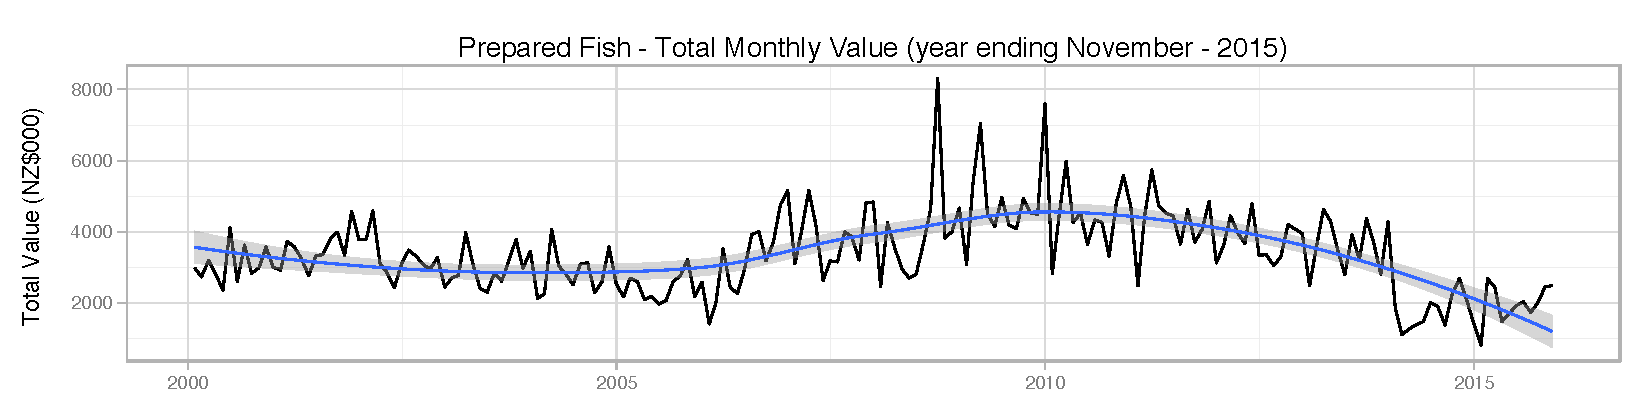
\includegraphics[scale=0.53]{../graphs/monthly_value/prepared_fish_monthly_value.pdf} \
    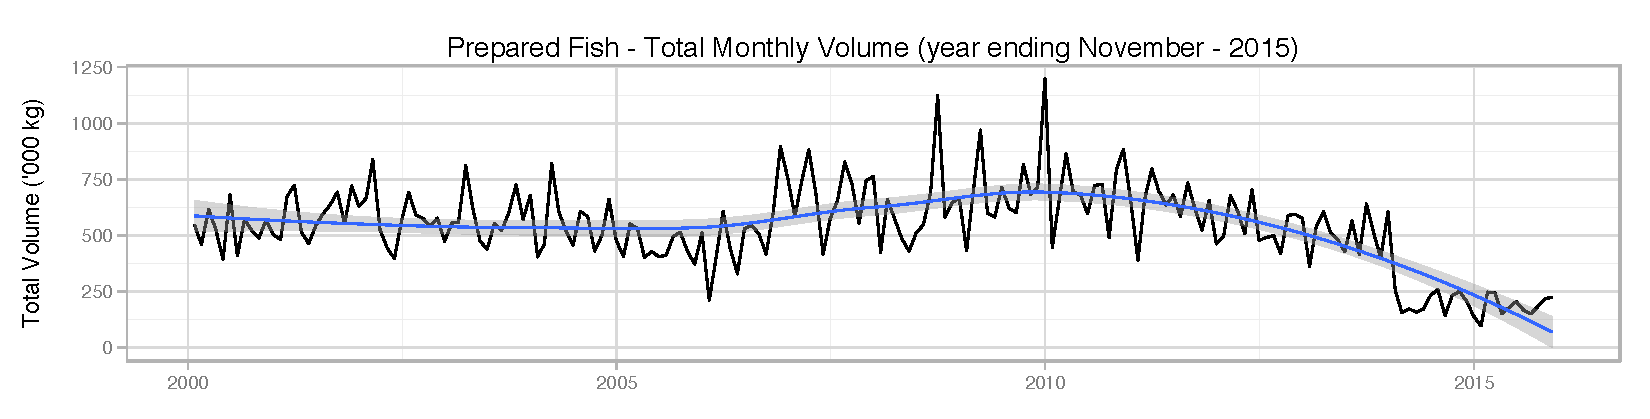
\includegraphics[scale=0.53]{../graphs/monthly_volume/prepared_fish_monthly_volume.pdf} \
    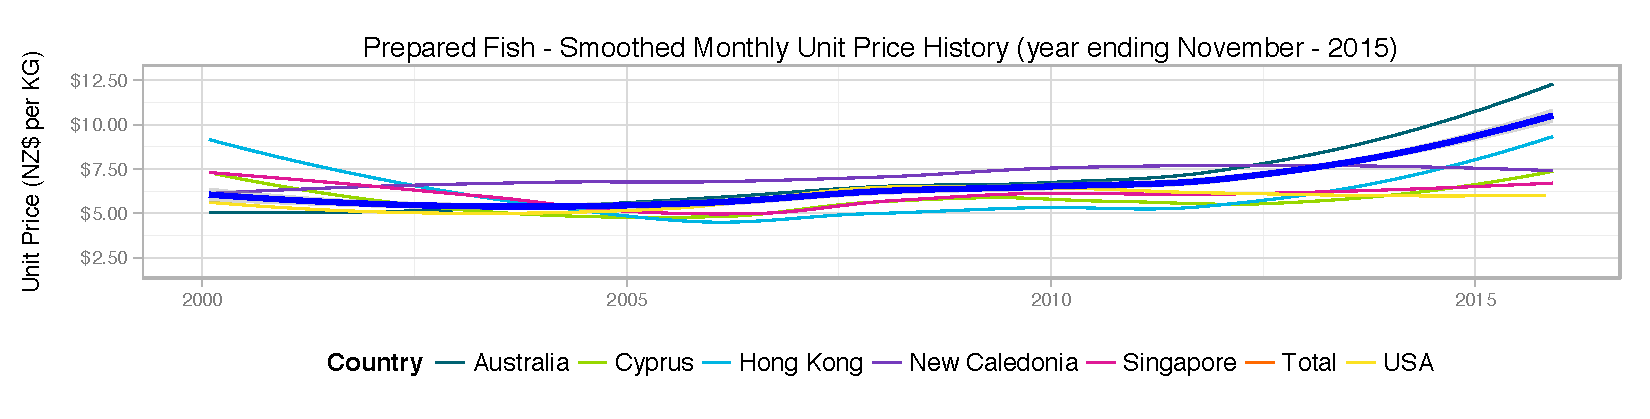
\includegraphics[scale=0.53]{../graphs/smoothed_price/prepared_fish_smoothed_price.pdf} \
    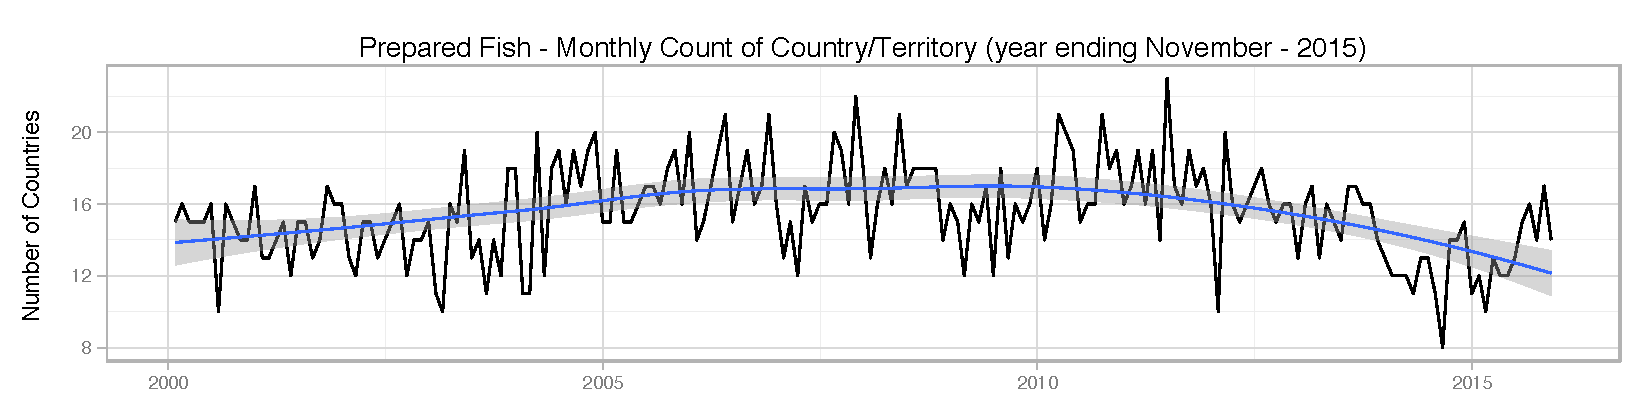
\includegraphics[scale=0.53]{../graphs/monthly_number_countries/prepared_fish_monthly_count.pdf} \
    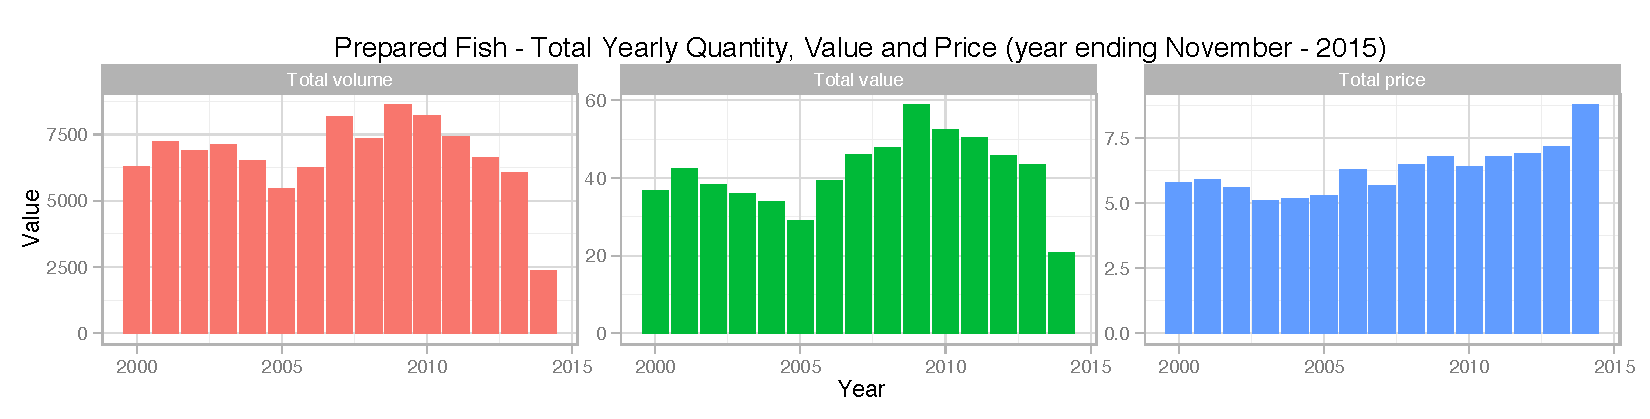
\includegraphics[scale=0.53]{../graphs/yearly_summary/prepared_fish_yearly_summary.pdf} \
   \end{figure}



\footnotetext[1]{Source: Statistics New Zealand - Overseas Merchandise Trade}
\footnotetext[2]{Harmonised System Codes for Prepared Fish starting with: 160419, 160420.}
\end{document}
